\section{Discussion}\label{sec:discuss}

In this work we have proposed a framework which extends Transformer models to 
naturally support types of relational learning, through cross-attention
mechanisms that enforce a relational bottleneck, so that only information about relations between encoder states
are used in transformations of the abstract states.
Building on insights gained from the implementation of a relational bottleneck in other forms \citep{esbn, kerg2022neural}, this exploits the powerful attentional capabilities of the transformer architecture to identify relevant relationships.
Experiments with sorting and other relational tasks indicate that this framework has the potential to combine the
benefits of function approximation over sensory states, as exploited in many deep learning models, with abstraction and relational reasoning abilities supported by symbolic processing.
Limitations of the current approach suggest interesting
future directions to better understand the potential of this framework, and
how it may relate to the algorithms of human cognition as implemented in the brain, opening up possibilities for 
improved alignment of natural and artificial intelligences.

Two directions to highlight are the use of external memories and attentional control. 
%The flexibility of transformer attention mechanisms comes with a computational and statistical price. An attention head over 
%$O(\m)$ objects incurs a quadratic $O(\m^2)$ cost to compute attention weights, and increasing $m$ and the number of attention heads results in language models with a large number of parameters, requiring large amounts of data to fit.
From a statistical perspective, the use of an external memory with relational cross attention effectively allows nonparametric and semiparametric models. To make this explicit, note that the classical kernel regression estimator for the Gaussian kernel
%given by
%\begin{align*}
%  \hat f(x) &= \frac{\sum_{i=1}^n \exp\left(-\frac{1}{2h^2} \|x-x_i\|^2\right) y_i}{\sum_{i=1}^n \exp\left(-\frac{1}{2h^2} \|x-x_i\|^2\right)} 
%  = \sum_{i=1}^n \alpha_i(x, x_{1:n}) y_i,
%\end{align*}
can be seen as relational cross-attention with relations and weights given by the kernel 
% with weights
%\begin{align*}
%    \alpha(x, x_{1:n}) &= \Softmax\left(\left\{-\frac{1}{2h^2}\|x-x_i\|^2\right\}\right) 
%    = \Softmax\left(\left\{\frac{1}{h^2}\langle x, x_i\rangle\right\}\right)
%\end{align*}
and values $y_{1:n}$. Viewed in terms of episodic memory, this has bindings $\{x_i\| y_i\}$ with values $y_i$ that 
might be seen as being stored on the abstract side if they are rewards or labels that are associated with 
a particular episode $x_i$. Under a learned relation, the model associates the reward with particular features or attributes of the inputs, as the kernel changes to compute relations as inner products $\langle W_Q x, W_K x_i \rangle$, leading to a semiparametric model. The number of keys grows unboundedly with the number of episodes experienced, while the query remains of constant size. Realizing this approach will allow a regulation of the bias-variance tradeoff through the way that attention is implemented, while limiting the number of parameters that need to be learned.

%\begin{figure}[t]
%    \vspace{-3mm}
%    \begin{center}
%    \begin{tabular}{c}
%        \hskip2pt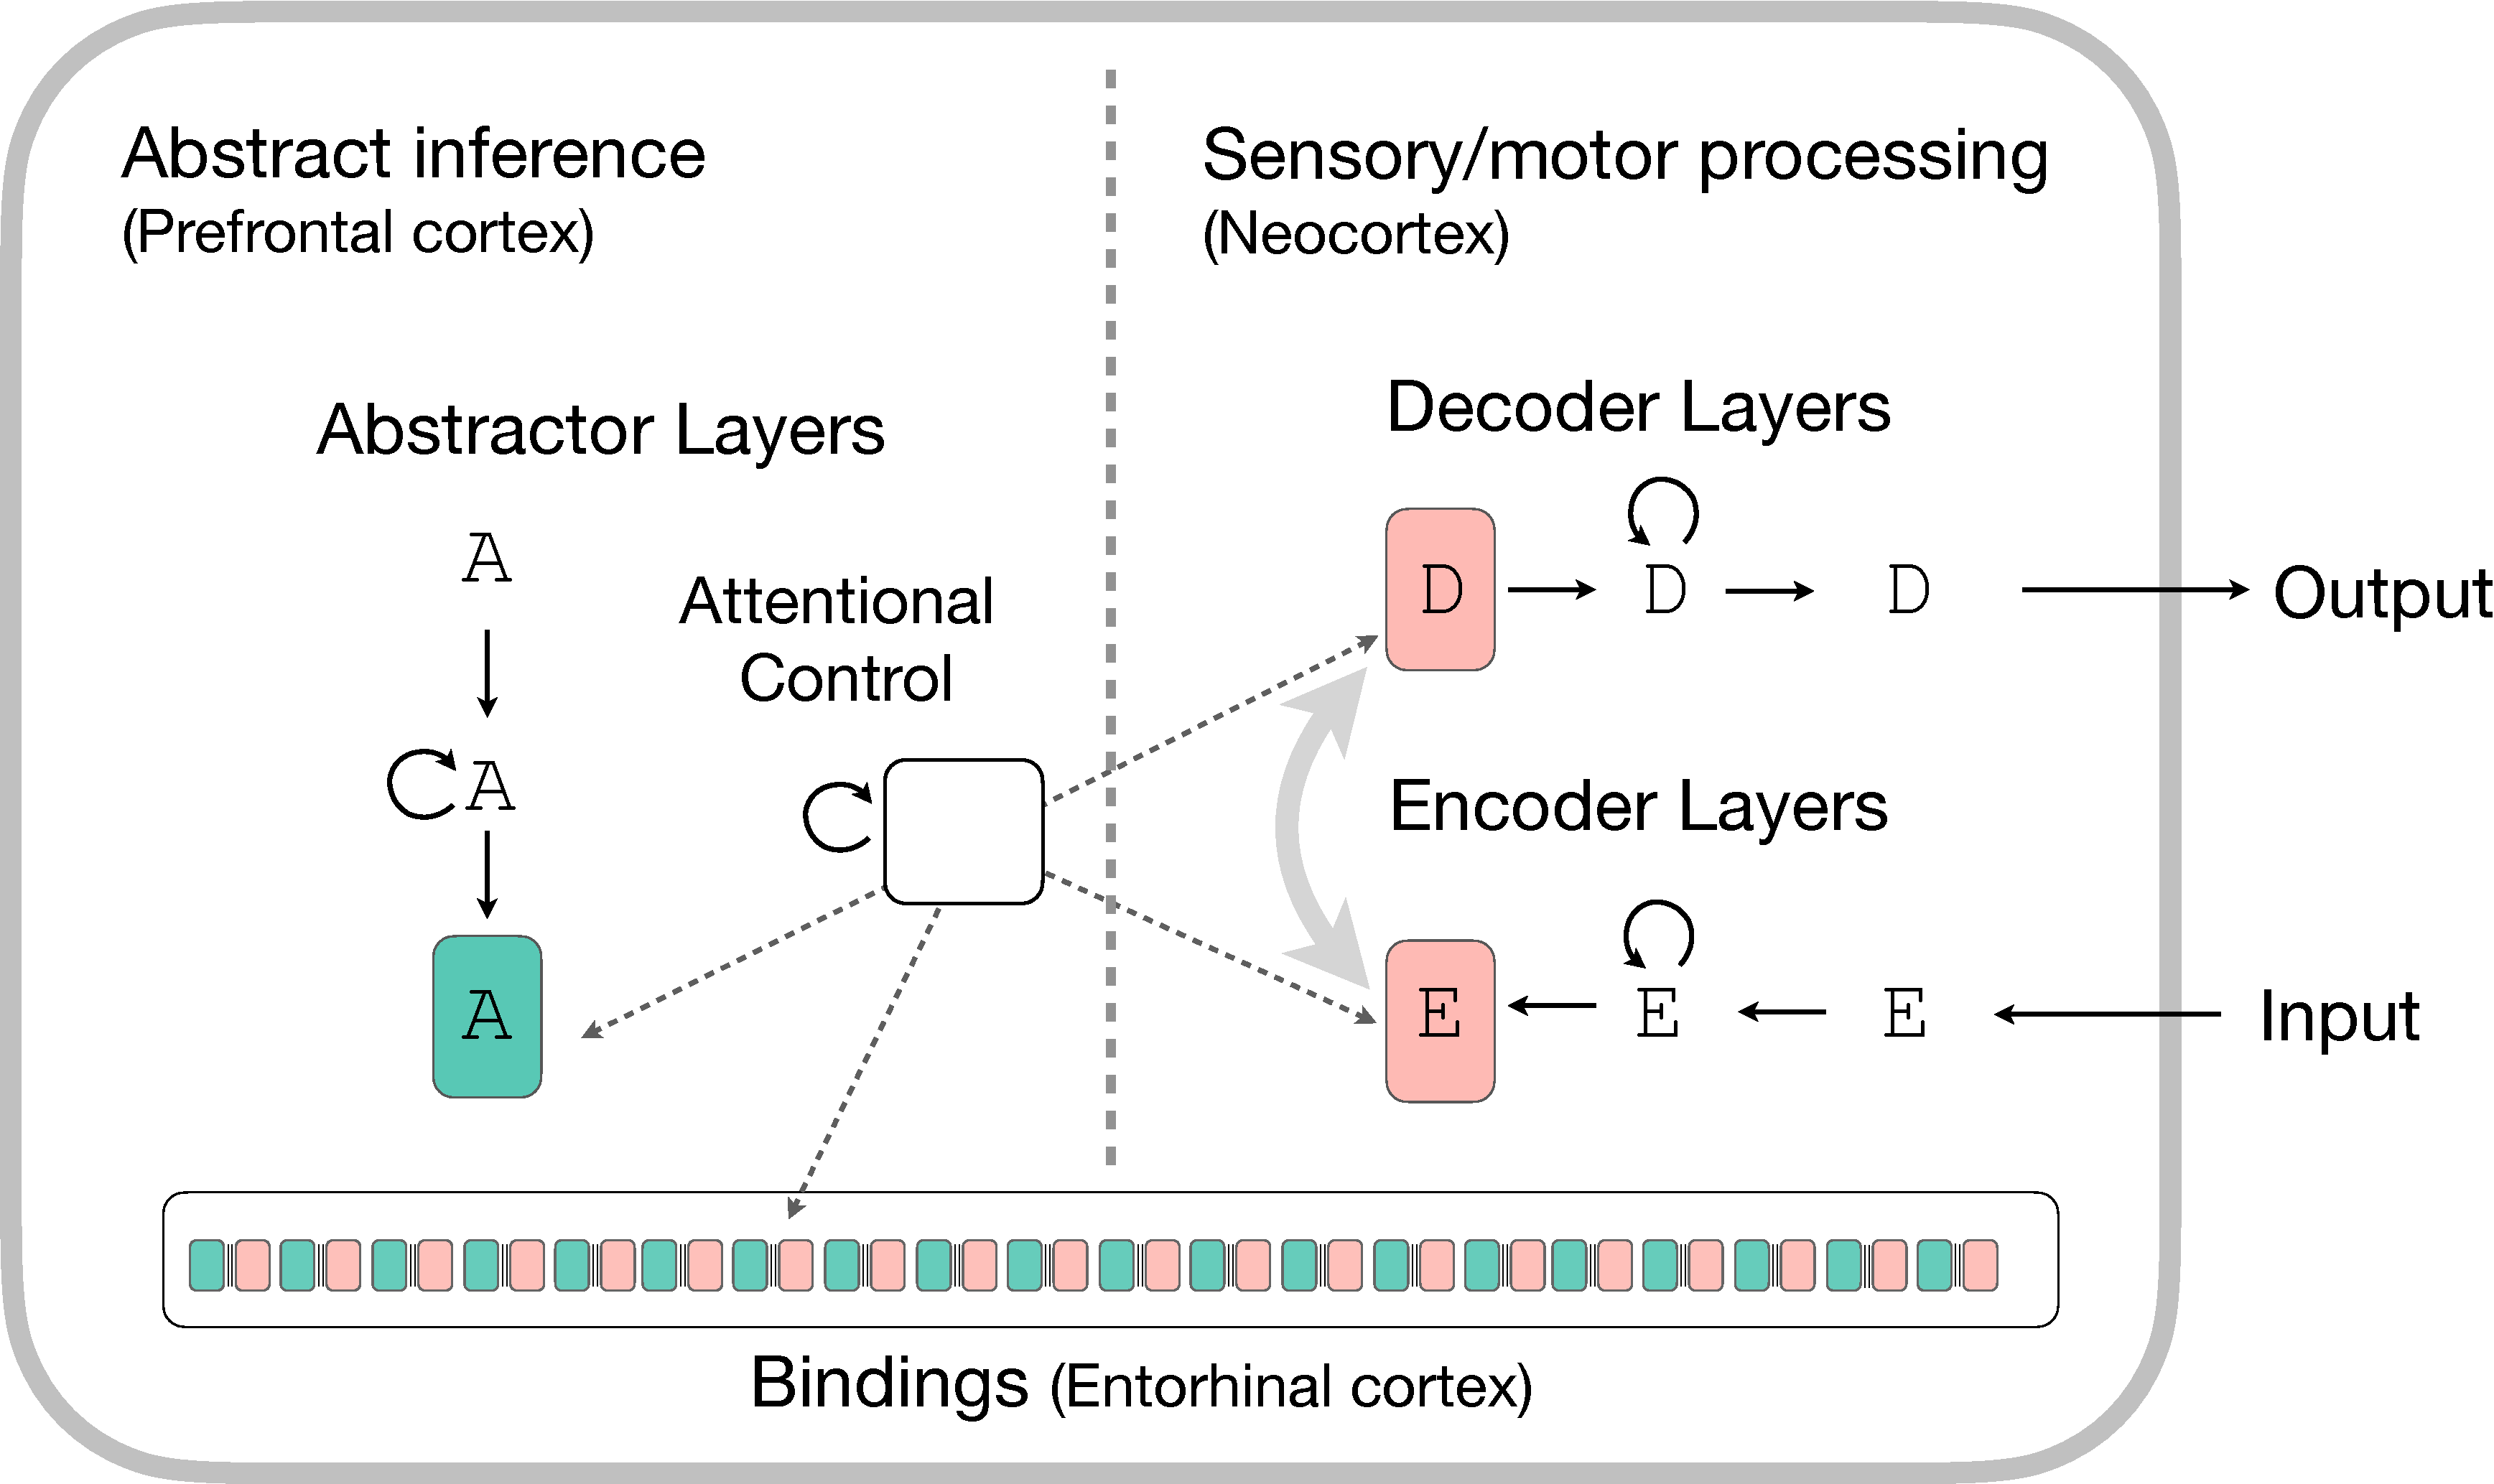
\includegraphics[width=.60\textwidth]{figures/algorithm-diagram2-crop} 
%    \end{tabular}
%    \caption{In a more general architecture, motivated by principles of information processing 
%    in the brain, the relational cross attention mechanisms can be regulated by a controller, and bindings between encoder/decoder and abstractor states are maintained in episodic memory. This allows abstract states to be shared and reused across problems and domains. When Encoder/Decoder states appear together repeatedly through experience and replay, the abstract inference circuit can be preempted by a direct connection (gray arrow), leading to computational efficiency and parallelization (i.e., consolidation and automatization).
%    }
%    \label{fig:algo2}
%    \vskip-12pt
%    \end{center}
%\end{figure}

A second direction, also motivated from cognitive neuroscience principles, is to replace 
parallel execution of attention heads with serial evaluation as directed by a controller. 
In standard transformers, attention operations are spread across multiple attention heads,
each of which is restricted in scope, and that are evaluated in parallel across GPUs by embedding them in matrix
multiplication. This is a powerful, but energy inefficient approach, which also reduces the pressure for learned
representations to be abstract and attentional operations to be generalizable, in ways that are exhibited
by the flexibility of human cognition.  It will be important to add a ``cognitive control'' mechanism that resides on
the abstract side and is responsible for selecting attention heads to be evaluated in each step in a serial fashion \citep{cohen2017cognitive}.  This could be seen as analogous to evaluative, gating and updating functions in anterior cingulate cortex, prefrontal cortex and basal ganglia
\citep{frank2001interactions,evc,braver2000control,wmPFC}
and implemented using neural network mechanisms such as LSTMs \citep{lstm} or variations on the transformer
architecture \citep{gamr}.


%While this more general framework would be designed to provide the flexibility of abstract, relational reasoning that
%can be generalized to novel inputs, it comes at the expense of control-dependent serial encoding and inference, which %can be avoided in cases where the stimuli and relationships among them are highly consistent. By allowing
%direct connections $E \Rightarrow D$ from encoder to decoder states to be learned if a task is repeated or replayed
%repeatedly, inferential abstract reasoning---which can be highly data efficient but relatively slow---can gradually
%be replaced by direct transformations between processing modules once a task is learned and repeatedly used, or
%internally replayed, corresponding to the process of automatization in humans that leads to more efficient, parallel
%processing \citep{schneider1977controlled, ravi2020navigating, musslick2021rationalizing}.  

